\documentclass[handout]{beamer}
\mode<presentation>
{
  \usetheme{Warsaw}
  \definecolor{utorange}{rgb}{1.0, 0.5098, 0}
  \definecolor{utwhite}{rgb}{1.0, 1.0, 1.0}
  \setbeamercolor{structure}{fg=utorange,bg=utwhite}
  \setbeamertemplate{frametitle}[default][shadow=false]
  %\setbeamercovered{transparent}
}


%\mode
%<handout>
%\usepackage{pgfpages}
%\pgfpagesuselayout{4 on 1}[letterpaper,border shrink=4mm]
%\setbeamertemplate{footline}[page number]



\usepackage[english]{babel}
\usepackage[latin1]{inputenc}
\usepackage{times}
\usepackage[T1]{fontenc}
\usepackage{tikz}
\usepackage{graphicx}
\usepackage[]{algorithm2e}
\usepackage{subfig}
\usepackage{amsmath}
\usepackage{amssymb}
\usepackage{mathrsfs}

\newcommand{\imagesource}[1]{{\centering\hfill\break\hbox{\scriptsize Image Source:\thinspace{\small\itshape #1}}\par}}

\title[Textual Influence Modeling]{Textual Influence Modeling Through Non-Negative Tensor Factorization}
\author{Robert Earl Lowe}

\date[]{July 12, 2018}
\subject{}

\pgfdeclareimage[height=0.5cm]{university-logo}{images/utklogo}
\logo{\pgfuseimage{university-logo}}



\AtBeginSection[]
{
  \begin{frame}<beamer>{Outline}
    \tableofcontents[currentsection]
  \end{frame}
}


\begin{document}
../commands.tex
\begin{frame}
  \titlepage
\end{frame}

\begin{frame}{Outline}
  \tableofcontents
\end{frame}

\section{Introduction}
\begin{frame}{Text Documents and Influences}
\begin{columns}
\column{0.5\textwidth}
\begin{itemize}[<+->]
  \item Every text document is a combination of an author's contributions and contributing factors.
  \item Contributing Factors
  \begin{itemize}
    \item Cited Sources
    \item Collaborators
    \item Unconcious Influences
  \end{itemize}
\end{itemize}

\column{0.5\textwidth}
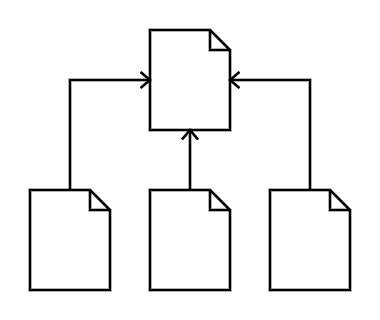
\includegraphics[width=\textwidth]{images/Citations}
\end{columns}
\end{frame}

\begin{frame}{Introduction to Tensors}
\begin{columns}
\column{0.7\textwidth}
\begin{itemize}[<+->]
\item Tensors are a generalization of matrices.
\item The number of {\em modes} of a tensor is the number of indices needed to address the tensor elements.
  \begin{itemize}[<+->]
  \item {\bf scalar} 0 modes
  \item {\bf vector} 1 mode
  \item {\bf matrix} 2 modes
  \item {\bf tensor} $>2$ modes
  \end{itemize}
\end{itemize}
\column{0.3\textwidth}
\begin{figure}
\centering
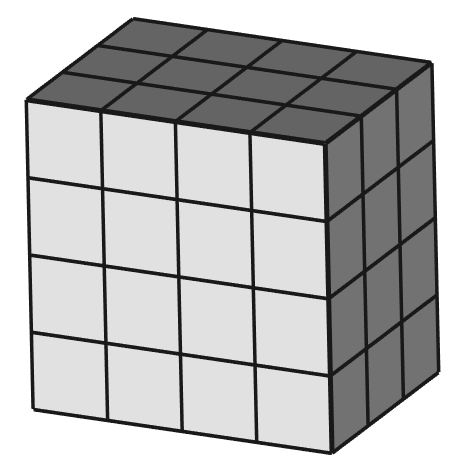
\includegraphics[width=\textwidth]{diagrams/tensor}
{\small A $4\times4\times3$ Tensor}
\end{figure}
\end{columns}
\end{frame}

\begin{frame}{Tensor Decompositions}
\begin{columns}
\column{0.6\textwidth}
Math Here
\column{0.4\textwidth}
\begin{figure}
  \centering
  \subfloat{
    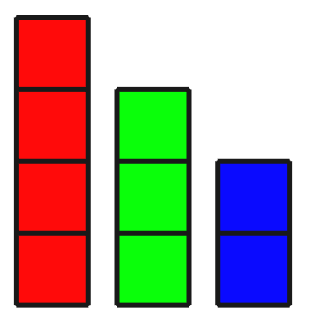
\includegraphics[height=0.25\textheight]{diagrams/mode_vectors}
  }
  \subfloat{
    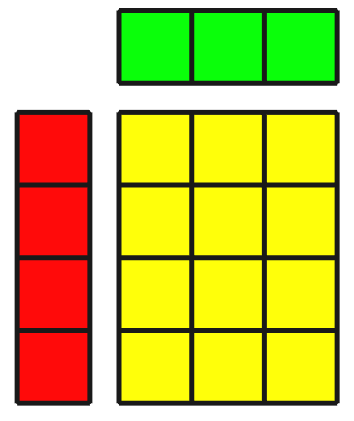
\includegraphics[height=0.25\textheight]{diagrams/mode1_tns_mode2}
  }\\
  \subfloat{
    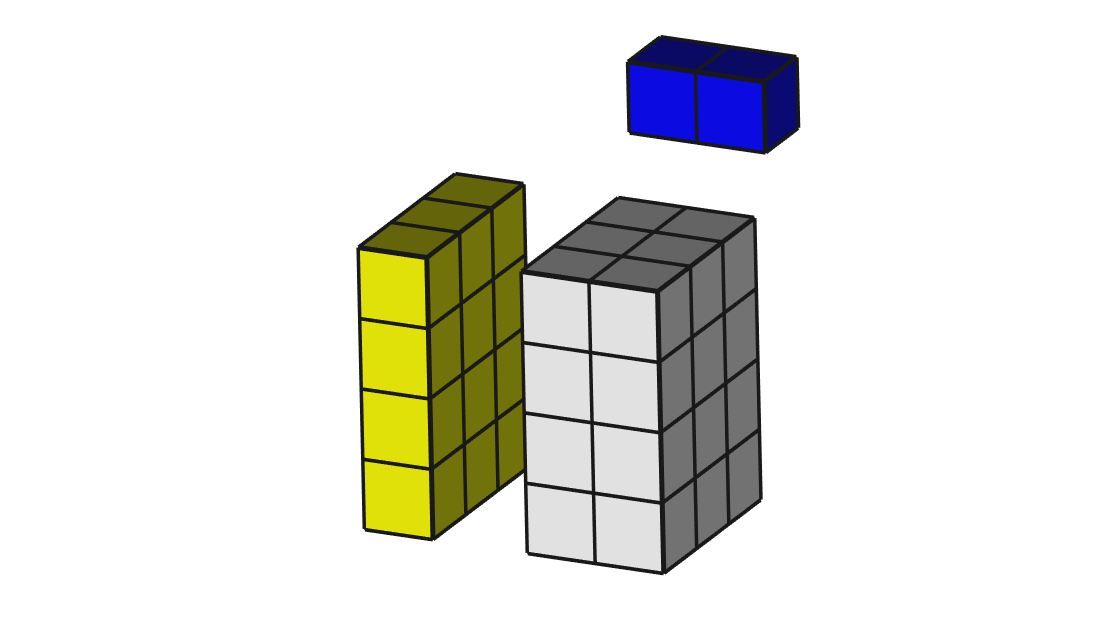
\includegraphics[height=0.25\textheight]{diagrams/mode12_tns_mode3}
  }
\end{figure}
\end{columns}
\end{frame}


\begin{frame}{Advantages of Tensor Decomposition}

\end{frame}


\begin{frame}{Representing Documents as Tensors}

\end{frame}


\begin{frame}{Non-Negative Decomposition of Document Tensors}

\end{frame}


\begin{frame}{Normalizing and Matching Document Components}

\end{frame}


\begin{frame}{Assigning Weights to Factors and Documents}

\end{frame}


\begin{frame}{Related Work}

\end{frame}


\section{Approach}
\begin{frame}{Overall Algorthm}
  \small
\begin{algorithm}[H]
  \caption{Influence Model Construction}
  \label{alg:model}

  \SetKwInOut{Input}{input}\SetKwInOut{Output}{output}
  \SetKwFunction{Prepare}{prepare}
  \SetKwFunction{BuildVocabulary}{build\_vocabulary}
  \SetKwFunction{BuildTensor}{build\_tensor}
  \SetKwFunction{ExtractFactors}{extract\_factors}
  \SetKwFunction{DistanceMatrix}{build\_distance\_matrix}
  \SetKwFunction{ExtractInfluence}{extract\_influence}
  \SetKwData{W}{$\set{W}$} \SetKwData{S}{$\set{S}$}
  \SetKwData{D}{$\tens{D}$}
  \SetKwData{V}{$\set{V}$} \SetKwData{LN}{$\Lambda$}
  \SetKwData{F}{$\set{F}$} \SetKwData{DM}{$M$}
  \SetKwData{C}{$\set{C}$}
  
  \Input{$docs$, $n$, $nfactors$, $threshold$}
  \Output{\W, \S, \F}
  \BlankLine
  \Prepare{$docs$}\;
  \V $\leftarrow$ \BuildVocabulary{$docs$}\;
  \C $\leftarrow\emptyset$\;
  \ForEach{$d$ in $docs$}{
    \D$ \leftarrow$ \BuildTensor($d$, $n$, $\set{V}$)\;
    $\C \leftarrow \C \cup \{\D\}$\;
  }
  \LN,\F $\leftarrow$ \ExtractFactors{\C, $nfactors$}\;
  \DM $\leftarrow$ \DistanceMatrix{\F}\;
  $\lambda \leftarrow$ the entries in \LN corresponding to the target document.\;
  \W, \S $\leftarrow$ \ExtractInfluence{$|docs|$, \DM,\F,$\lambda$, $threshold$}\;
  \Return{\W, \S, \F}\;
\end{algorithm}
\end{frame}


\begin{frame}{Corpus Preparation}
\begin{algorithm}[H]
  \caption{Prepare}
  \label{alg:Prepare}
  \SetKwInOut{Input}{input}\SetKwInOut{Output}{output}
  \Input{$docs$}
  \Output{None}
  \BlankLine
  \ForEach{$d$ in $docs$}{
    Remove Punctuation from $d$\;
    Remove Numbers from $d$\;
    Convert $d$ to lower case\;
  }
\end{algorithm}
\end{frame}


\begin{frame}{Vocabulary Extraction}
\begin{algorithm}[H]
  \caption{Build Vocabulary}
  \label{alg:vocabulary}
  \SetKwInOut{Input}{input}\SetKwInOut{Output}{output}
  \SetKwData{V}{$\set{V}$}
  \Input{$docs$}
  \Output{\V}
  \BlankLine
  $\V\leftarrow\emptyset$\;
  \ForEach{$d$ in $docs$}{
    \ForEach{$word$ in $d$}{
      $\V \leftarrow \V \cup \{word\}$\;
    }
  }
  \Return{\V};
\end{algorithm}
\end{frame}


\begin{frame}{Building Document Tensors}
  \small
\begin{algorithm}[H]
  \caption{Build Tensor}
  \label{alg:BuildTensor}
  \SetKwData{D}{$\tens{D}$} \SetKwData{V}{$\set{V}$} \SetKwData{N}{$n$}
  \SetKwInOut{Input}{input}\SetKwInOut{Output}{output}
  
  \Input{$d$, $n$, \V, \N}
  \Output{\D}
  \BlankLine
  $\D \leftarrow $ Tensor with dimension $|\V| \times |\V| \ldots
  \times_n |\V|$\;
  Fill \D with 0\;
  $len \leftarrow$ number of words in $d$\;
  \For{$i \leftarrow 1 $ to $len - n$} {
    \tcc{Compute Tensor Element Index}
    $index \leftarrow$ list of $n$ integers\;
    \For{$j\leftarrow i $ to $i+n$} {
      $index[j] \leftarrow$ index of word $d[j]$ in \V\;
    }
    \tcc{Update Frequency of This $n$-gram}
    $\D[index] \leftarrow \D[index] + 1$\;
  }
  \Return{\D}
\end{algorithm}
\end{frame}


\begin{frame}{Tensor Decomposition}
  \tiny
  \begin{algorithm}[H]
  \label{alg:ExtractFactors}
  \caption{Extract Factors}
  \SetKwData{LN}{$\Lambda$}  \SetKwData{C}{$\set{C}$}
  \SetKwData{F}{$\set{F}$} \SetKwData{U}{$\set{U}$}
  \SetKwData{T}{$\tens{T}$}\SetKwData{D}{$\tens{D}$}
  \SetKwFunction{Norm}{$\mathrm{L}_1$\_norm}
  \SetKwFunction{CCD}{ccd\_ntfd}
  \SetKwInOut{Input}{input}\SetKwInOut{Output}{output}
  \Input{\C, $nfactors$}
  \Output{\LN, \F}
  \BlankLine
  $\F \leftarrow \emptyset$\;
  $\LN \leftarrow \emptyset$\;
  $nmodes \leftarrow$ number of modes in $\C[1]$\;
  \ForEach{\D in \C}{
    $\U \leftarrow $ \CCD{\D, $nfactors$}\;
    \For{$i$ = 1 to $nfactors$}{
      \tcc{Build the Factor}
      $\T \leftarrow \U[1][:,i]$\;
      \For{$m$ = 2 to $nmodes$}{
        $\T \leftarrow \T \otimes \U[m][:,i]$\;
      }

      \tcc{Compute the norm and normalize the factor}
      $\lambda \leftarrow $\Norm{\T}\;
      $\T \leftarrow \T / \lambda$\;

      \tcc{Insert the factor and norm into the list}
      $\F \leftarrow \F \cup \{\T\}$\;
      $\LN \leftarrow \LN \cup \{\lambda\}$\;
    }
  }
  \Return{\LN, \F}
\end{algorithm}
\end{frame}


\begin{frame}{Distance Computation}
\begin{algorithm}[H]
  \caption{Build Distance Matrix}
  \label{alg:distance}
  \SetKwData{DM}{$M$} \SetKwData{F}{$\set{F}$}
  \SetKwInOut{Input}{input}\SetKwInOut{Output}{output}
  \SetKwFunction{Norm}{$\mathrm{L}_1$\_norm}
  \Input{\F}
  \Output{\DM}
  \BlankLine
  $\DM \leftarrow $ Matrix with dimension $|\F| \times |\F|$\;
  \For{$i=1$ to $|\F|$}{
    \For{$j=1$ to $|\F|$} {
      $\DM[i,j] \leftarrow$ \Norm{$\F[i] - \F[j]$}\;
    }
  }
  \Return{\DM}
\end{algorithm}
\end{frame}


\begin{frame}{Factor Matching }
\tiny
\begin{algorithm}[H]
  \caption{Extract Influence}
  \label{alg:influence}
  \SetKwInOut{Input}{input}\SetKwInOut{Output}{output}
  \SetKwData{DM}{$M$} \SetKwData{F}{$\set{F}$}
  \SetKwData{LN}{$\set{\lambda}$}\SetKwData{Ndocs}{$ndocs$}
  \SetKwData{W}{$\set{W}$} \SetKwData{S}{$\set{S}$}
  
  \Input{\Ndocs, \DM, \F, \LN, $threshold$}
  \Output{\W, \S}
  \BlankLine
  \tcc{Compute Weights}
  $s \leftarrow \sum \LN$\;
  $\W \leftarrow \LN / s$\;
  \BlankLine
  \tcc{Classify Factors}
  $nfactors \leftarrow |\LN|$\;
  \For{$i=1$ to $nfactors$}{
    $min \leftarrow \DM[row,1]$\;
    $minIndex \leftarrow 1$\;
    $row \leftarrow i + nfactors * (ndocs-1)$\;
    \For{$j=1$ to $nfactors * ndocs$}{
      \If{\DM[row,j]$< min$}{
        $min \leftarrow \DM[row,j]$\;
        $minIndex \leftarrow j$\;
      }
    }
    \eIf{$min \leq threshold$}{
      $\S[i]\leftarrow minIndex$\;
    }{
      $\S[i]\leftarrow 0$\;
    }
  }
  \Return{\W, \S}\;
\end{algorithm}
\end{frame}


\begin{frame}{Final Summation}
\begin{algorithm}[H]
  \caption{Final Summation}
  \label{alg:summation}
  \SetKwInOut{Input}{input}\SetKwInOut{Output}{output}
  \SetKwData{F}{$\set{F}$}
  \SetKwData{LN}{$\set{\lambda}$}\SetKwData{Ndocs}{$ndocs$}
  \SetKwData{W}{$\set{W}$} \SetKwData{S}{$\set{S}$}
  \SetKwData{I}{$\set{I}$} \SetKwData{Author}{$author$}
  
  \Input{\Ndocs, \S, \W}
  \Output{\I, \Author}
  \BlankLine
  $\I \leftarrow $ List of 0 repeated $\Ndocs-1$ times
  \For{i = 1 to \Ndocs} {
    \eIf{$\S[i] = 0$} {
      $\Author = \Author + \W[i]$
    }{
      $j \leftarrow $ Document number corresponding with $\S[i]$
      $\I[j] \leftarrow \I[j] + \W[i]$
    }
  }
\end{algorithm}
\end{frame}


\begin{frame}{Implementation}

\end{frame}


\section{Results}
\begin{frame}[t]{A Simple Example: Cat and Dog}
\begin{columns}[T]
  \column{0.33\textwidth}
  \begin{block}{The Cat's Tale}
    \small
    The cat sat on the mat.  The cat was happy to be on the mat.  The
    cat saw the mouse running but was too lazy to chase it.
  \end{block}
  \column{0.33\textwidth}
  \begin{block}{The Dog's Tale}
    \small
    The dog walked to the house.  The dog saw the food bowl, and the
    dog saw a squirrel.  The dog chased the squirrel from the food
    bowl.
  \end{block}
  \column{0.33\textwidth}
  \begin{block}{The Saga Continues}
    \small
    The dog saw the cat on the mat.  The dog walked to the house, and
    the dog chased the cat.  The squirrel was happy to see the dog
    chase the cat on the mat.  The dog saw the squirrel, and decided
    to chase the squirrel instead.  The cat sat on the mat.
  \end{block}
\end{columns}
\end{frame}


\begin{frame}{Cat and Dog Vocabulary and Tensors}

  \begin{columns}[T]
    \column{0.5\textwidth}
    \begin{table}
      \centering
      \tiny
      {\bf Vocabulary}\\
      \begin{tabular}{c|l||c|l}
        $I$ & Word & $I$ & Word\\ 
        \hline
        1 & the & 16 & chased \\
        2 & house & 17 & sat \\
        3 & mouse & 18 & be \\
        4 & squirrel & 19 & happy \\
        5 & it & 20 & on\\
        6 & saw & 21 & from \\
        7 & lazy & 22 & food \\
        8 & cat & 23 & decided \\
        9 & mat & 24 & to\\
        10 & a & 25 & was \\
        11 & bowl & 26 & dog \\
        12 & walked & 27 & running \\
        13 & too & 28 & instead \\
        14 & and & 29 & but \\
        15 & see & 30 & chase\\
      \end{tabular}
    \end{table}
    \column{0.5\textwidth}
    \begin{table}
      \tiny
      {\bf Non-Zero Entries of Cat Tensor}\\
      \begin{tabular}{rrr|r}
        $i$ & $j$ & $k$ & $freq$\\
        \hline
        1&8&17&1\\
        8&17&20&1\\
        17&20&1&1\\
        20&1&9&2\\
        1&9&1&2\\
        9&1&8&2\\
        1&8&25&1\\
        8&25&19&1\\
        25&19&24&1\\
        19&24&18&1\\
        24&18&20&1\\
        18&20&1&1\\
        1&8&6&1\\
        8&6&1&1\\
        6&1&3&1\\
        1&3&27&1\\
        3&27&29&1\\
        27&29&25&1\\
        29&25&13&1\\
        25&13&7&1\\
        13&7&24&1\\
        7&24&30&1\\
      \end{tabular}
    \end{table}
\end{columns}
\end{frame}


\begin{frame}{Cat and Dog Model Parameters and Output}
  \begin{columns}[T]
    \column{0.5\textwidth}
    \begin{table}
      \centering
      \tiny
      Model Parameters\\
      \begin{tabular}{ll}
        \hline
        $n$-gram size & 3\\
        \hline
        $nfactors$ &  7 \\
        \hline
        $threshold$ & 0.2\\
        \hline
        Corpus Size & 3\\
        \hline
        Total Word Count & 107\\
        \hline
      \end{tabular}
    \end{table}

  \column{0.5\textwidth}
  \begin{table}
    \centering
    \tiny
    Model Output\\
    \begin{tabular}{|l|c|l|}
      \hline
      Factor & Factor Weight & Classification\\
      \hline
      1 & 0.28 & Author Contribution\\
      \hline
      2 & 0.15 & Cat Factor 1\\
      \hline
      3 & 0.14 & Author Contribution\\
      \hline
      4 & 0.14 & Author Contribution\\
      \hline
      5 & 0.11 & Author Contribution\\
      \hline
      6 & 0.11 & Author Contribution\\
      \hline
      7 & 0.06 & Dog Factor 1\\
      \hline
    \end{tabular}
  \end{table}
  \small
  \begin{table}
    \begin{tabular}{ll}
      Author Contribution & 0.79\\
      Cat Contribution & 0.15\\
      Dog Contribution & 0.06\\
    \end{tabular}
  \end{table}
\end{columns}
\end{frame}


\begin{frame}{Cat and Dog Influencing Factors}
  \begin{columns}
    \column{0.5\textwidth}
    \small
    \begin{table}
      \centering
      \tiny
      Matched to Cat Factor 1\\
      \begin{tabular}{lll|r}
        Word 1 & Word 2 & Word 3 & Proportion\\
        \hline
        on & the & mat & 1.00\\
      \end{tabular}
    \end{table}
    \column{0.5\textwidth}
    \small

    \begin{table}
      \centering
      \tiny
      Matched to Dog Factor 1\\
      \begin{tabular}{lll|r}
        Word 1 & Word 2 & Word 3 & Proportion\\
        \hline
        the & dog & saw & 0.40\\
        the & dog & walked & 0.20\\
        the & dog & chased & 0.20\\
        the & dog & chase & 0.20\\
      \end{tabular}
    \end{table}
  \end{columns}
\end{frame}


\begin{frame}{Cat and Dog Original Factors}
  \begin{columns}[T]
    \column{0.5\textwidth}
    \begin{table}
      \tiny
      \begin{tabular}{lll|r}
        Word 1 & Word 2 & Word 3 & Proportion\\
        \hline
        saw & the & squirrel & 0.267417\\
        saw & the & cat & 0.223651\\
        saw & the & dog & 0.192194\\
        cat & the & squirrel & 0.044066\\
        cat & the & cat & 0.036854\\
        cat & the & dog & 0.031670\\
        mat & the & squirrel & 0.034331\\
        mat & the & cat & 0.028712\\
        mat & the & dog & 0.024674\\
        see & the & squirrel & 0.032132\\
        see & the & cat & 0.026873\\
        see & the & dog & 0.023094\\
        chased & the & squirrel & 0.013437\\
        chased & the & cat & 0.011238\\
        chased & the & dog & 0.009657\\
        \hline
        squirrel & and & happy & 0.249836\\
        squirrel & and & decided & 0.262960\\
        squirrel & was & happy & 0.237368\\
        squirrel & was & decided & 0.249836\\
        \hline
      \end{tabular}
    \end{table}
    \column{0.5\textwidth}
    \begin{table}
      \tiny
      \begin{tabular}{lll|r}
        Word 1 & Word 2 & Word 3 & Proportion\\
        \hline
        decided & to & chase & 1.000000\\
        \hline
        happy & to & see & 1.000000\\
        \hline
        cat & saw & the & 0.345830\\
        cat & see & the & 0.040819\\
        cat & chased & the & 0.172914\\
        cat & chase & the & 0.213734\\
        walked & saw & the & 0.056987\\
        walked & see & the & 0.006726\\
        walked & chased & the & 0.028493\\
        walked & chase & the & 0.035220\\
        to & saw & the & 0.044398\\
        to & see & the & 0.005240\\
        to & chased & the & 0.022199\\
        to & chase & the & 0.027439\\
        \hline
      \end{tabular}
    \end{table}
\end{columns}
\end{frame}

\begin{frame}{Case Study: Regional Conference Paper}
  \begin{table}
    \centering
    \tiny
    Corpus of Scientific Papers\\
  \begin{tabular}{|l|l|}
    \hline
    1 & Jessica Lin, Eamonn Keogh, Stefano Lonardi, and Bill Chiu. A\\
      & symbolic representation of time series, with implications
        for\\
      & streaming algorithms.  ACM Press, 2003\\
    \hline
    2 & Andreas Schlapbach and Horst Bunke. Usinghmm\\
      & based recognizers for writer identification and
        verficiation.\\
      & IEEE, 2004\\
    \hline
    3 & Yusuke Manabe and Basabi Chakraborty. Identy\\
      & detection from on-line handwriting time series.\\
      & IEEE, 2008\\
    \hline
    4 & Sami Gazzah and Najoua Ben Amara. Arabic handwriting \\
      & texture analysis for writer identification using the \\
      & dwt-lifting scheme.  IEEE, 2007.\\
    \hline
    5 & Kolda, Tamara Gibson. Multilinear operators for higher-order \\
      & decompositions. 2006\\
    \hline
    6 & Blei, David M and Ng, Andrew Y and Jordan, Michael I. Latent\\
      & dirichlet allocation. 2007\\
    \hline
    7 & Serfas, Doug. Dynamic Biometric Recognition of Handwritten Digits\\
      & Using Symbolic Aggregate Approximation. Proceedings of the ACM\\
      & Southeast Conference 2017\\
    \hline
  \end{tabular}
\end{table}
\end{frame}


\begin{frame}{Model Parameters}
    \begin{table}
      \centering
      Model Parameters\\
      \begin{tabular}{ll}
        \hline
        $n$-gram size & 3\\
        \hline
        $nfactors$ &  150 \\
        \hline
        $threshold$ & 0.2\\
        \hline
        Corpus Size & 7\\
        \hline
        Total Word Count & 45,152\\
        \hline
      \end{tabular}
    \end{table}
\end{frame}


\begin{frame}{Influence and Original Factors}
  \begin{columns}[T]
    \column{0.4\textwidth}
    \begin{table}
      \tiny
      \centering
      \begin{tabular}{|l|c|l|}
        \hline
        Document & Influence & Factors\\
        \hline
        1 & 0.21 & 10\\
        2 & 0.09 & 9\\
        3 & 0.06 & 3\\
        4 & 0.06 & 1\\
        5 & 0.00 & 0\\
        6 & 0.00 & 0\\
        Author & 0.57 & 127\\
        \hline
      \end{tabular}
    \end{table}
    \column{0.7\textwidth}
    Information From Reading the Target Paper
    \begin{itemize}[<+->]
      \item The first cited source details the algorithm which the
        author extends.  The factors pulled from this source all
        discuss the properties of the original algorithm.
      \item The second, third, and fourth cited sources are previous
        algorithms, to which the new one is compared.
      \item Papers five and six are from a completely unrelated field.
      \end{itemize}
    \end{columns}
\end{frame}


\begin{frame}{Distribution of All Factor Distances}
  \begin{figure}
    \centering
    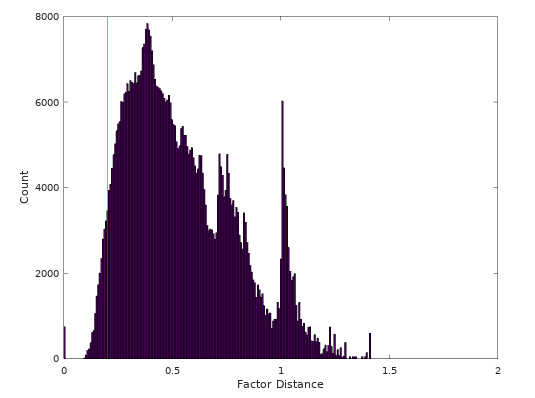
\includegraphics[height=0.6\textheight]{diagrams/conference-factor-distance}
  \end{figure}
\end{frame}


\begin{frame}{Distribution of Target Factor Distances}
  \begin{figure}
    \centering
    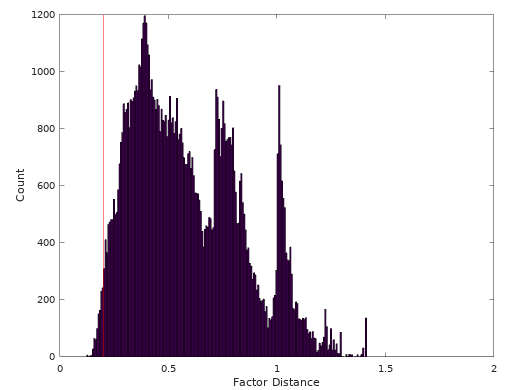
\includegraphics[height=0.6\textheight]{diagrams/conference-target-distance}
  \end{figure}
\end{frame}


\begin{frame}{Conclusion and Future Work}

\end{frame}


\begin{frame}{Bibliography}

\end{frame}


\end{document}